\section{Problem Statement}
Suppose there exists an arbitrary number of robots in a dynamic indoor environment. Also suppose there exists a series of decentralized cameras arranged in a grid layout with overlapping field of views between neighboring cameras. The objective is to dynamically and simultaneously provide guidance to all robots to safely reach their destinations.

\subsection{Assumptions}
For this work, it is assumed that the ground robots have Collision Detection capabilities, allowing them to stop if a collision were incoming. This potential collision could be with another robot or a person.

It is also assumed that a waypoint graph has been built in each region overseen by a camera such that any path covers clear ground exclusively. Methods for generating a waypoint graph have been discussed in \cite{WaypointJia} and \cite{WaypointVideoGames}.

\subsection{Definitions}

We define an environment for our system which resembles an industrial storage facility. This environment is dynamic and arbitrary. Our system consists of a set of ceiling-mounted smart cameras and a set of robots. 

A set of ceiling-mounted smart cameras view the entire working region of the environment, where an individual camera can see a small subset of the entire environment. Each camera has a working region which has slight overlap with all of its neighbors. These cameras are arranged in a grid in order to simplify this neighboring region overlap. The set of cameras are decentralized such that there is no central server performing any of the processing. For simplicity, each camera is mounted at the same height and each camera's region is the same size. At start-up, each camera performs an initialization phase which calculates a waypoint graph that represents its region.

Within the system, there exists a set of robots. After camera initialization, the robots received arbitrary instructions from a human user which tell the robot where to go (a goal which, in an industrial setting, would be where it would pick-up or drop-off cargo). The robots do not move synchronously. 

There exists middleware for communication between all agents in the system - camera-to-camera, robot-to-robot, robot-to-camera, and camera-to-robot. This communication is necessary for decentralization so that each agent can retrieve any information it requires.

% FIXME: need to better describe this image in this section FIXME %
\begin{figure}[!t]
\centering
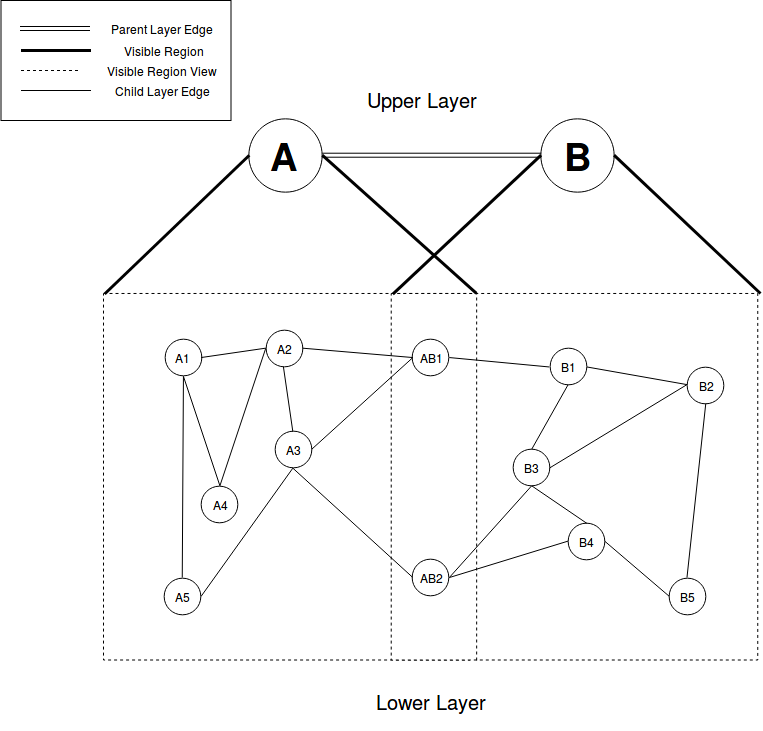
\includegraphics[width=3in]{HierarchicalSystem}
\caption{Simplified hierarchical network of nodes.}
\label{fig_hier}
\end{figure}

From here, we can decompose our system into a hierarchical graph where each region within a camera will be a set of child-layer nodes and each camera will be a parent-layer node. That is, each camera will be a parent to a set of nodes that exist within the waypoint graph of its region. Furthermore, each camera will have siblings that correspond to the neighboring cameras. This can be seen in figure \ref{fig_hier}. This figure shows a system containing two parent nodes, \{\(A,B\)\}. These nodes represent a ceiling-mounted smart camera in the physical system. Each of these parent nodes contains a set of child nodes, \{\(A1, A2, A3, A4, A5, AB1, AB2\)\} and \{\(B1, B2, B3, B4, B5, AB1, AB2\)\} respectively. Each child layer contains the points \{\(AB1, AB2\)\} which are therefore defined as overlap points as they are shared between parents.

We can define our upper-level system as an undirected graph, \(G = (V,E)\), where \(V\) is the set of cameras and where \(E\) defines the set of all edges that represent a pair of neighboring cameras. We further define our lower-level system as an undirected graph, \(G' = (V',E')\), where \(V'\) is the set of all waypoint nodes within each camera and where \(E'\) is the set of all edges that represent a pair of waypoint nodes. For each camera \(V_i\), there exists a set of child nodes \(C_i\).
We can declare a pair of cameras neighbors with the equation
\begin{equation}
\forall V_i, V_j \in V \ \exists E(V_i, V_j) \iff C_i \cap C_j \neq \varnothing
\end{equation}
Using this equation, it stands that neighbors have a set of overlapping points such that
\begin{equation}
O_{i,j} =  C_i \cap C_j
\end{equation} 
We then define a camera \(V_i\)'s unique set of child nodes to be 
\begin{equation}
P_i = C_i - \sum_j O_{i,j}
\end{equation}


We define our set of robots as \(R = \{ R_1, ..., R_k \}\) where the number of robots does not exceed \(V(G')\). The set of robots travel along the nodes of the lower-level graph, \(G'\). 

\subsection{Proposed Solution}
Current solutions to indoor robot navigation require a static environment in which calculations are performed by either a central server or the robots. In the case of robots performing calculations, each robots needs a local version of the entire map. If the environment is dynamic, it could be expensive to update the map of every robot. If the environment is dynamic, most solutions are ineffective or inefficient. 
I propose a solution that utilizes the performance of a decentralized system and handles dynamic environments in an efficient manner. 

This sytem uses an array of decentralized ceiling-mounted smart cameras covering the entirety of the map. Once the region is mapped, robots request a path from a source camera to a goal camera. Each camera may interact with with any other camera to incrementally build a path. Two version of A* were designed in this work. In the first, all processing is done on the source camera who will request information from any other camera in the system. In the second, the processing is done on the camera whose region is being checked. After it has finished the necessary processing, it will send required information back to the source camera. 
